%Przykładowy plik ułatwiający złożenie projektu dyplomowego inżynierskiego.
%UWAGA: Generowany napis na stronie tytułowej o treści PROJEKT DYPLOMOWY INŻYNIERSKI został zaproponowany przeze mnie i nie jest, póki co, potwierdzony przez władze wydziału. Przed ostatecznym oddaniem tak złożonej pracy należy upewnić się jaka powinna być treść tego napisu. W momencie gdy uzyskam informację na temat treści tego napisu, dokonam niezbędnych zmian w źródłach.

\documentclass[eng,printmode]{mgr}
%opcje klasy dokumentu mgr.cls zostały opisane w dołączonej instrukcji

%poniżej deklaracje użycia pakietów, usunąć to co jest niepotrzebne
%\usepackage{polski} %przydatne podczas składania dokumentów w j. polskim
\usepackage{polski}
\usepackage[utf8]{inputenc}
\usepackage[T1]{fontenc} %poprawne składanie polskich czcionek
%pakiety do grafiki
\usepackage{graphicx}
\usepackage{subfigure}
\usepackage{psfrag}

%pakiety dodające dużo dodatkowych poleceń matematycznych
\usepackage{amsmath}
\usepackage{amsfonts}

%pakiety wspomagające i poprawiające składanie tabel
\usepackage{supertabular}
\usepackage{array}
\usepackage{tabularx}
\usepackage{hhline}
\usepackage{multirow}
%pakiet wypisujący na marginesie etykiety równań i rysunków zdefiniowanych przez \label{}, chcąc wygenerować finalną wersję dokumentu wystarczy usunąć poniższą linię
%\usepackage{showlabels}


%definicje własnych poleceń
\newcommand{\R}{I\!\!R} %symbol liczb rzeczywistych, działa tylko w trybie matematycznym
\newtheorem{theorem}{Twierdzenie}[section] %nowe otoczenie do składania twierdzeń

%dane do złożenia strony tytułowej
\title{System lokalizacji samolot\.'ow z wykorzystaniem ADS-B}
\engtitle{Airplane tracking system using ADS-B}
\author{Karol Szpila}
\supervisor{\vfil dr in\.z. Krzysztof Halawa\\
\\ Katedra Informatyki Technicznej}
%\guardian{dr hab. inż. Imię Nazwisko Prof. PWr, I-6} %nie używać jeśli opiekun jest tą samą osobą co prowadzący pracę

%\date{2008} %standardowo u dołu strony tytułowej umieszczany jest bieżący rok, to polecenie pozwala wstawić dowolny rok

%poniżej jest lista kierunków i specjalności na wydziale elektroniki, należy wybrać właściwe lub dopisać jeśli nie ma odpowiednich
\field{Automatyka i Robotyka (AIR)}
\specialisation{Technologie Informacyjne\\ w Systemach Automatyki (ART)}
%\specialisation{Robotyka (ARR)}
%\specialisation{Komputerowe sieci sterowania (ARK)}
%\specialisation{Systemy informatyczne w automatyce (ASI)}
%\specialisation{Komputerowe systemy zarządzania \\procesami produkcyjnymi (ARS)}
%\field{Elektronika i telekomunikacja (EIT)}
%\specialisation{Akustyka (ETA)}
%\specialisation{Aparatura elektroniczna (EAE)}
%\specialisation{Elektroniczne i komputerowe \\systemy automatyki (ESA)}
%\specialisation{Zastosowania inżynierii komputerowej \\w technice (EZI)}
%\specialisation{Inżynieria dźwięku (EID)}
%\specialisation{Elektronika stosowana \\i optokomunikacja (TEO)}
%\specialisation{Telekomunikacyjne sieci szerokopasmowe (TSS)}
%\specialisation{Teleinformatyczne sieci mobilne (TSM)}
%\specialisation{Sygnały w telekomunikacji cyfrowej (TSC)}
%\specialisation{Teleinformatyczne systemy rozsiewcze (TSR)}
%\field{Informatyka (INF)}
%\specialisation{Systemy informatyki w medycynie \\i technice (IMT)}
%\specialisation{Inżynieria systemów informatycznych (INS)}
%\specialisation{Inżynieria internetowa (INT)}
%\specialisation{Systemy i sieci komputerowe (ISK)}
%\field{Teleinformatyka (TIN)}
%\specialisation{Teleinformatyka (TIN)}

%tutaj zaczyna się właściwa treść dokumentu
\begin{document}
%\bibliographystyle{plabbrv} %tylko gdy używamy BibTeXa, ustawia polski styl bibliografii

\maketitle %polecenie generujące stronę tytułową
%\dedication{6cm}{To jest przykładowa treść opcjonalnej dedykacji, należy ją zmienić lub usunąć w całości polecenie \texttt{$\backslash$dedication}}

\tableofcontents %spis treści

%poniżej znajduje się przykładowa treść dalszej części dokumentu, zainteresowanych zachęcam do rozszyfrowania frazy "Lorem ipsum" :)
\let\cleardoublepage\clearpage %usuwa puste strony pomiaedzy rozdziałami

\chapter{ Wstęp }
ADS-B (ang. Automatic Dependent Surveillance–Broadcast) to system służący do śledzenia statków powietrznych wykorzystywany w kontroli ruchu powietrznego. Powstał, aby uzupełniać pracę PSR (ang. Primary Surveilance Radar) i w przyszłości go całkowicie zastąpić. PSR to radar aktywny bazujący na wysyłaniu fal elektromagnetycznych oraz pomiarze czasu powrotu fali odbitej od obiektu. Wadą takich systemów jest brak informacji o wykrytym obiekcie poza jego lokalizacją i rozmiarem, wrażliwość na ukształtowanie terenu oraz warunki pogodowe. ADS-B bazuje na lokalizacji przy pomocy satelit GPS. Statki powietrzne w sposób ciągły ustalają swoją pozycję oraz nadają drogą radiową swoje położenie, prędkość oraz identyfikator.
\\


Mode-S to system SSR (ang. Secondary Surveillance Radar) wykorzystywania do odpytywania statku powietrznego o danym 24-bitowym adresie ICAO (ang International Civil Aviation Organization). SSR to wtórny radar dozorowania, uzupełniający prace PSR o dodatkowe informacje odebrane od statku powietrznego. Zapytania wysyłane są przez ATM (ang. Air Traffic Management) na częstotliwości 1030Mhz, natomiast odpowiedzi na 1090Mhz.ADS-B wykorzystuje Mode-S jako technologię do przesyłania informacji.

\begin{table}[ph]
\caption{\textit{ Rodzaje wiadomości ADS-B}}
\label{tab:adsb}
  \centering
  \def\arraystretch{1.3}% 
  \begin{tabular}{|c|c|c|}
  \hline
  \multicolumn{1}{|c|}{Rodzaj wiadomości} & \multicolumn{1}{c|}{Downlink Format} & \multicolumn{1}{c|}{Zawartość} \\\cline{1-3}
  \multirow{4}{*}{ADS-B (56 bitów)} 
  				 & \multicolumn{1}{c|}{DF0} & \multicolumn{1}{c|}{Odpowiedz Short Air to Air ACAS} \\\cline{2-3}
                 & \multicolumn{1}{c|}{DF4} & \multicolumn{1}{c|}{Poziom lotu} \\\cline{2-3}
                 & \multicolumn{1}{c|}{DF5} & \multicolumn{1}{c|}{Identyfikator (Roll-call)} \\\cline{2-3}
                 & \multicolumn{1}{c|}{DF11} & \multicolumn{1}{c|}{Mode-S odpowiedz All-call} \\\hline
  \multirow{6}{*}{ADS-B (112 bitów)} 
  				 & \multicolumn{1}{c|}{DF16} & \multicolumn{1}{c|}{Odpowiedz Long Air to Air ACAS} \\\cline{2-3}
                 & \multirow{5}{*}{DF17} & Pozycja powietrzna \\\hhline{~~~} 
                 &                       & pozycja lądowa \\\hhline{~~~} 
                 &                       & status \\\hhline{~~~} 
                 &                       & ID i rodzaj samolotu  \\\hhline{~~~} 
                 &                       & prędkość powietrzna \\\hline
 \multirow{2}{*}{Mode-S EHS (112 bitów)} 
	& \multicolumn{1}{c|}{DF20} & \multicolumn{1}{c|}{Poziom lotu oraz (BDS 4.0/5.0/6.0)} \\\cline{2-3}
	& \multicolumn{1}{c|}{DF21} & \multicolumn{1}{c|}{ID oraz (BDS 4.0/5.0/6.0)} \\\hline
 \end{tabular}
\end{table}
\newpage

Powyższa tabela prezentuje podział wiadomości ADS-B ze względu na rozmiar bloku danych oraz DF (ang. Downlink Format), czyli format odebranej ramki. Wiadomosci można podzielić według długości bloku danych na normalne o długości 56 bitów i rozszerzone 112 bitowe.DF0 i DF16 wykorzystywane są w ACAS (ang. Airborne Collision Avoidance System).Wyróżniamy odpowiedz Short air to air ACAS (DF0), odbieran przez stacje ATM, oraz Long air to air ACAS (DF16), stosowaną do informowania poszczególnych statków o możliwości kolizji. Statki wysyłające ramkę DF5 potwierdzają, że są wyposarzone w transponder ADS-B. Ponadto, można wyróżnić odpowiedzi Mode-S EHS (ang. Enhanced Surveillance) DF20 i DF21, uzyskiwanie na zapytanie kontroli naziemnej, które zawierają dodatkowe informacja niedostępne w Mode-S ADS-B, w zależności od wysłanego przez kontrolę naziemną BDS (ang. Comm-B Data Selector). BDS to numer określający żądaną w odpowiedzi informację. Tylko SSR który wysłał zapytanie Mode-S EHS jest wstanie zdekodować otrzymaną odpowiedź DF20 i DF21, poniewąż nie zawiera on wysłanego BDS. Poniżej przedstawiono tabelę z wymienionymi wcześniej BDS.

\begin{table}[ph]
\caption{\textit{ Rodzaje wiadomości ADS-B}}

  \centering
  \begin{tabular}{l}
  \\
    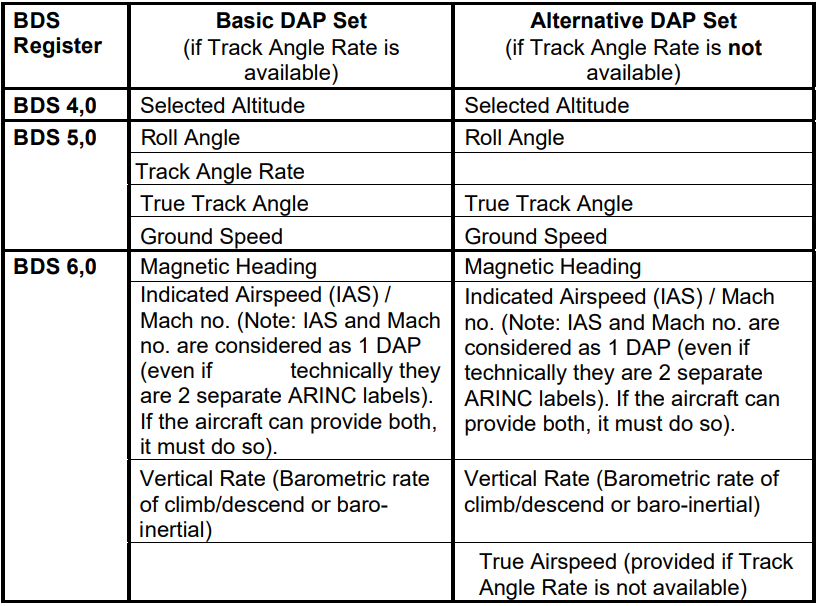
\includegraphics[width=\textwidth]{images/bds.png}
 \end{tabular}
\end{table}

Wiadomość ADS-B i Mode-S EHS można odbierać przy pomocy dowolnego odbiornika dostrojonego do częstotliwości 1090MHz. Tunery z układem RTL2832U o można łatwo przekształcić w SDR (ang. Software Defined Radio) SDR to system komunikacji radiowej w którym można stroić poprzez pogram bez ingerencji w sprzęt. Wspomniany odbiornik jest znacznie tańszy od profesjonalnych rozwiązań, co zpopularyzowało ADS-B w zastosowaniach amatorskich. 



%Transfer danych w Mode-S odbywa się z prędkoscią 1Mb/s, a ramki są modulowanie przy pomocy PPM (ang Pulse Position Modulation). PPM w przypadku sygnału cyfrowego polega na 



\chapter{ Cele i założenia projektowe }
Celem niniejszej pracy by\l{}o zbudowanie prototypu systemu pozwalającego na lokalizację oraz zbieranie informacji o  statkach powietrznych wyposażonych w transpondery ADS-B.


%System zostanie zbudowany w oparciu o mikrokontroler z rodziny STM32F7 ze względu na parametry sprzętowe i peryferia. 
%Jako radio do odbierania wiadomości ADS-B zostanie wykorzystany tuner DVB-T USB ze względu na niską cenę oraz gotowe biblioteki pozwalające łatwo przekształcić urządzenie w SDR (ang. Software Defined Radio). SDR to programowalne radio które można dostroić do obierania zadanej częstotliwości bez ingerencji w sprzęt. Wykorzystane zostaną do tego biblioteki STM32 USB Host i rtlsdr. Urządzenie zostanie wyposażone w wyświetlacz prezentując zebrane dane jako                                                                                                                                                                                                                                                                                                                                            obraz radaru z pozycją samolotu względem systemu oraz tabelą z informacjami dodatkowymi. Wykorzystana zostanie do tego biblioteka STemWin bedąca dedykowaną wersją emWin dla mikrokontrolerów ST.
\chapter{ Realizacja projektu }
\section{ Schemat Urządzenia}
W tym rozdziale zostanie opisana czę\'s\'c sprzętowa projektu, czyli schemat urządzenia oraz projekt PCB, wykorzystane elementy oraz zewnętrzne urządzenia.
\subsection{Zasilanie}
Urządzenie jest zasilanie z zewnętrznego źródła 5V poprzez port USB typu mini A. Pozwala to na podłącznie PCB zarówno do sieci przy pomocy ładowarki do telefonu jak i z komputera czy z przenośnego power banku. Ponieważ układy takie jak mikrokontroler czy pamieć SDRAM potrzebują napięcia 3.3V zastosowano stabilizator LM1117 Poniżej przedstawiono schemat podłączania.

\begin{figure}[!h]
    \centering
    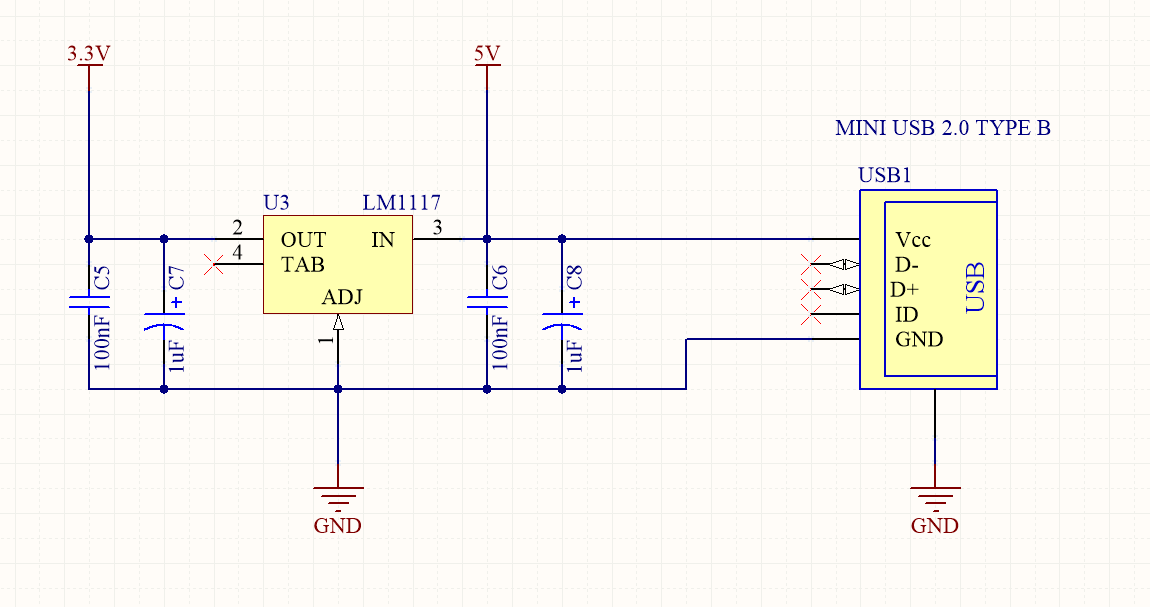
\includegraphics[width=\textwidth]{schematics/power.png}
    \caption{\textit{\scriptsize Schemat zasilania płZytki PCB}}
\end{figure}
\subsection{Mikrokontroler}
Wykorzystany mikrokontroler to STM32F767ZIT6. Układ został wybrany ze względu na zmieszczenie w najmniejszej obudowie wszystkich wymaganych układów peryferiów takich jak: kontroler LDTC do sprzętowej obsługi wyświetlacza LCD, kontroler pozwalający obsłużyć zewnętrzną pamięcią SDRAM i interfejsy komunikacyjne USB, I2C i UART. Poniżej przedstawiono schemat podłączenia.

\begin{figure}[!h]
    \centering
    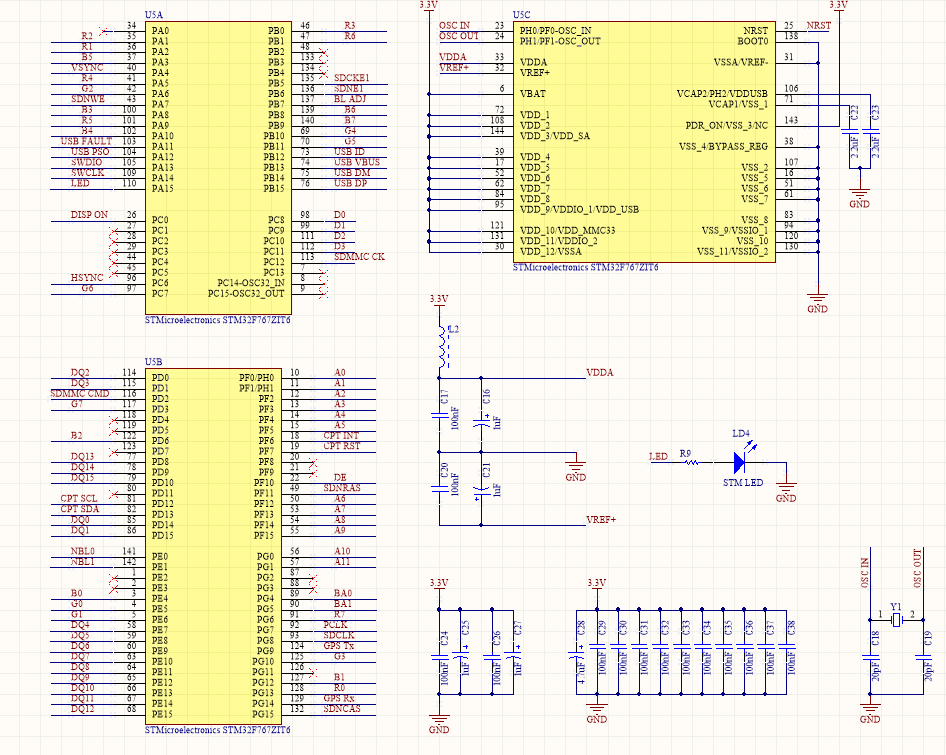
\includegraphics[height=\textwidth, angle=90]{schematics/uC.png}
    \caption{\textit{\scriptsize Schemat podłączenia mikrokontrolera STM32f767ZIT6}}
\end{figure}

\subsection{Interfejsy komunikacyjne}
System posiada gniazdo na kartę Micro SD, która może zostać wykorzysta do przechowywania skompresowanych obrazów do tła GUI lub co planowane jest w przyszłości map pozwalających lepiej orientować się w terenie na podstawie obrazu z radaru. Do programowania mikrokontrolera wykorzystany został dedykowany dwuprzeowodowy interfejs SWD zgodny z ST-Link. Ostatni zostanie omówiony interfejs USB do komunikacji z SDR (eng Software Defined Radio). Interfejs został wyprowadzony poprzez gniazdo Micro USB-B pozwalając w ten sposób zaoszczędzić miejsca na PCB. System jako Host USB będzie zasilać podłączony układy których pobór nie powinien przekroczyć, zgodznie ze stangardem USB2.0 500mA ,dlatego zastosowano power switch STMPS2141STR. W przypadku podania stanu wysokiego na pin USB PSO switch zostanie właczony. Jeżeli nie występują żadne sytuacje nieporządne takie jak przetężenie prądowe czy zwarcie, zapali się zielona dioda sygnalizująca poprawnie działanie zasilania. W przypadku jakichkolwiek problemów prąd zostanie natychmiast odcięty a układ wystawi wysoki stan na pin FAULT informując mikrokontroler i zapalając czerwona diodę. W celu zabezpieczania interfejsu przed nieporządanymi wyładowaniami elektrostatycznymi związanymi z dotykaniem urządzenia czy wkładaniem urządzenia do gniazda zastosowano układ ochrony ESD (ang . Electro Static Discharge ) STMECMF02-4CMX8 dedykowany dla USB2.0. Poniżej przedstawiono schemat połacznia na PCB.
 %sprawdzic czy prawda z h na faul

\begin{figure}[!h]
    \centering
    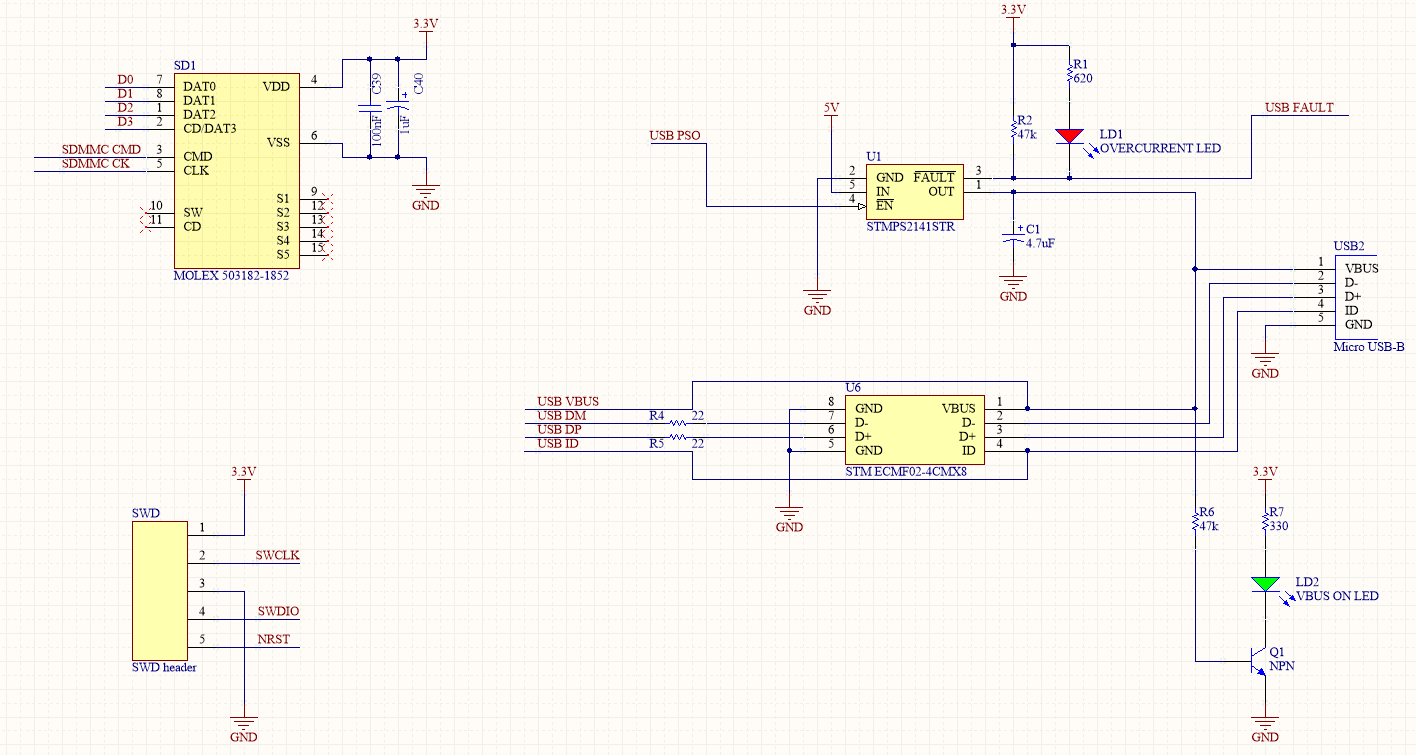
\includegraphics[width=\textwidth]{schematics/conn.png}
    \caption{\textit{\scriptsize Schemat podłączenia zewnętrych interfejsów}}
\end{figure}

\subsection{Wyświetlacz}
Zgodnie z założeniem, system ma posiadać interfejs graficzny dla użytkownika. Do tego celu wybrano wyświetlacz HY101CTP o przekątnej 10,1" i rozdzielczości 1024 na 600 pikseli. Matryca jest sterowana poprzez MIPI-DPI (ang. Mobile Industry Processor Interface - Display Parell Interface) 24bity na pikesl przy użyciu wbudowanego w układ STM32F7 kontrolara LTDC. Panel dotykowy komunikuje się z mikrokontrolerem poprzez interfejs I2C. Rezystory R3 i R8 mają za zadanie wymusić stan wysoki na liniach, ponieważ są sterownie w trybie otwartego drenu. W tej konfiguracji można tylko zewrzeć linie do masy zmieniając stan wysoki na niski. Pozwoliło to wyeliminować sytuacje w której linia na jednym końcu jest zwarta do masy a na drugim do zasilania co doprowadziło by do zwarcia i gwałtownego wzrostu mocy mogącego uszkodzić układ.
\begin{figure}[!h]
    \centering
    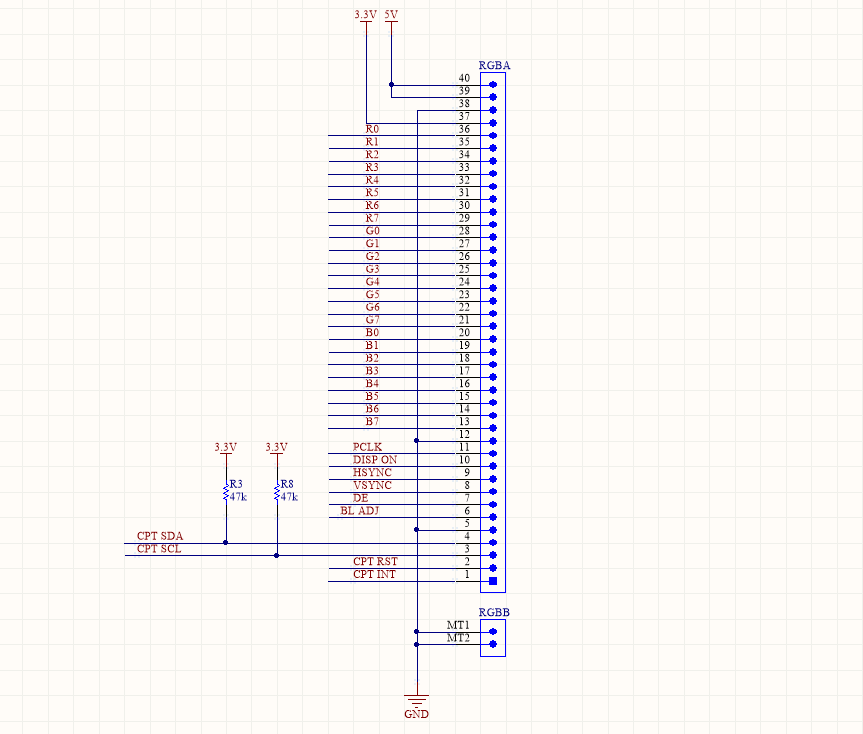
\includegraphics[width=\textwidth]{schematics/display.png}
    \caption{\textit{\scriptsize Schemat podłączenia wyswietlacza}}
\end{figure}

\subsection{SDRAM}
Do działania interfejsu graficznego potrzebna jest pamięć do przechowywania ramek wysyłanych do wyświetlacza poprzez interfejs MIPI-DPI. Założono iż warstwy będą przechowywane w pamięci w formacie ARGB8888 (po bajcie na każdy kolor i kanał alfa). Kontroler LTDC jest w stanie sprzętowo mieszać dwie warstwy w wynikową która jest wysyłana do wyświetlacza. Zdecydowano, że potrzeba pamięci wystarczająco dużej, by zmieścić trzy bufory. Pierwsza warstwa byłaby przeznaczony na tło, które jest niezmienne podczas działania urządzenia. Dwie pozostałe warstwy służyłby do naprzemiennej prezentacji zmiennych danych takich jak położenie statku powietrznego. Będzie to implementacja mechanizmu podwójnego buforowania pozwalająca wyeliminować migotanie matrycy podczas modyfikacji bufora aktualnie wyświetlanego. Trzy warstwa o rozmiarze 1024 na 600 piskeli w formacie ARGB8888 zajmą 57600 Kb. W pracy zdecydowano się wykorzystać układ IS42S16400J-7TLI posiadający 65536 Kb pamięci. Poniżej przedstawiono schemat połączenia z mikrokontrolerem.

\begin{figure}[!h]
    \centering
    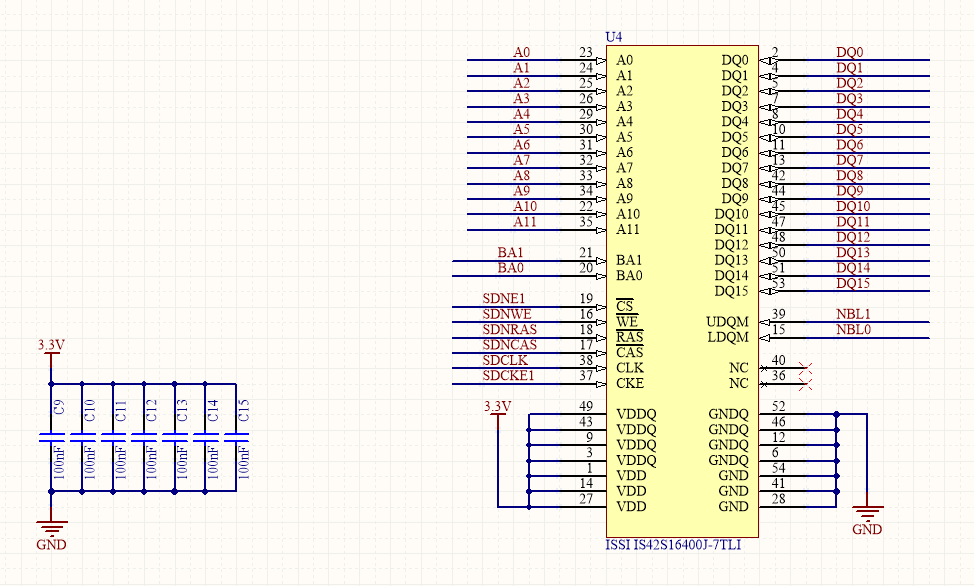
\includegraphics[width=\textwidth]{schematics/sdram.png}
    \caption{\textit{\scriptsize Schemat podłączenia zewnętrzej pamięci SDRAM}}
\end{figure}

\subsection{Moduł GPS}
Aby system był w stanie popranie obliczyć odległość od namierzonego statu powietrznego i poprawnie zaznaczyć jego pozycję na radarze, potrzebna znać pozycje urządzenia. Do tego zadania wybrano układ NEO-6M-0-001 z zewnętrzną aktywną anteną. Do układu została podłączono zewnętrza bateria podtrzymująca zasilanie. Dzieki temu urządzenie może uruchomić poprzez ciepły start, co pozwala zaoszczędzić czas potrzebny na znalezienie odpowiedniej liczby satelit Do komunikacji z mikrokontrolerem wybrano interfejs UART.

\begin{figure}[!h]
    \centering
    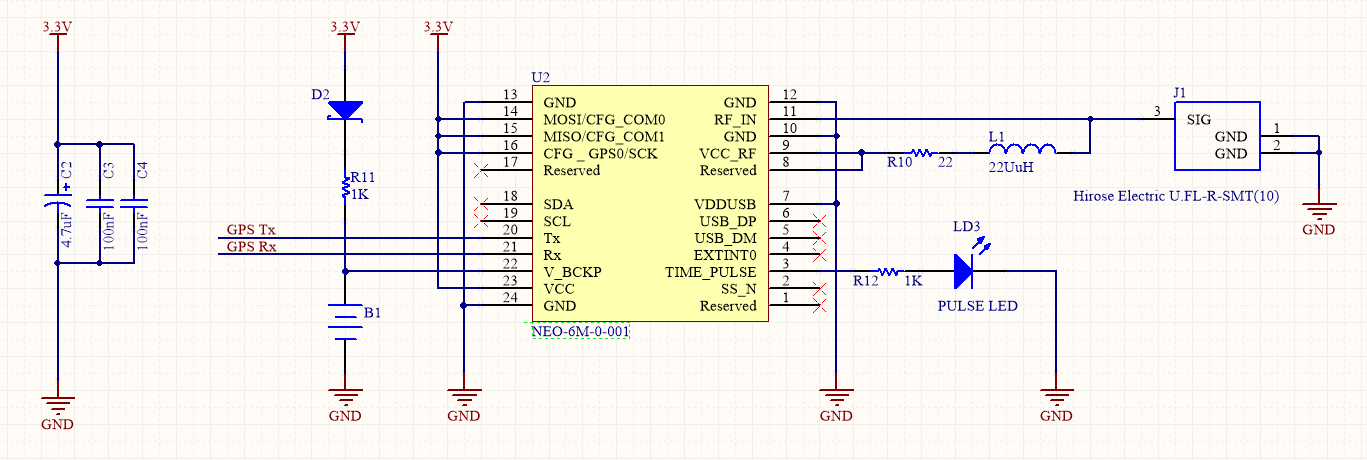
\includegraphics[width=\textwidth]{schematics/gps.png}
    \caption{\textit{ Schemat podłączenia modułu GPS}}
\end{figure}
\newpage

\section{ Wykonanie PCB }
W tym rozdziale szczegółowo opisano projekt oraz parametry wykonanego PCB. Pokazano obliczenia uzasadniające decyzje projektowe oraz ograniczenia wynikające z technologi produkcji i zastosowanych układów. 

\subsection{Parametry PCB} \label{pcbSection}
W projekcie PCB zdecydowano się na wykonanie technologia czterowarstwową. Pozwoliło to zmniejszyć rozmiary urządzenia oraz zapewnić dobre ekranowanie dla pomiędzy warstwami sygnałowymi. Ograniczyło to przesłuchy pomiędzy warstwami. Ponadto ciągłość warstw referencyjnych (masy i zasilania) pozwala by prądy powrotne przepływało możliwe najkrótszą drogą o najmniejszej impedancji zmniejszając emisje EMC. Poniżej przedstawiono tabele z układem warstw PCB.

\begin{table}[htb]

\caption{\textit{ Kolejność i grubość warst PCB}}
\label{tab:pcbStack}
\begin{center}
\begin{tabular}{ |c|c|c|c| }
\hline
Warstwa& grubość [mm] & grubość [mil] \\ 
\hline
sygnały & 0.03556 & 1,4 \\ 
\hline
dielektryk & 0,17018 & 6,7\\ 
\hline
masa & 0,01778 & 0,7\\ 
\hline
rdzeń & 1,1938 & 47\\ 
\hline
zasilanie & 0,01778 & 0,7\\ 
\hline
dielektryk & 0,17018 & 6,7\\ 
\hline
sygnały & 0.03556 & 1,4 \\ 
\hline
\end{tabular}
\end{center}
\end{table}

Warstwy przewodzące wykonane są z miedzi natomiast jako dielektryk wykorzystano materiał FR-408 o stałej dielektrycznej \textbf{$\varepsilon_r$} = 3.66

\subsection{GPS}
Zgodnie z notą katalogową układu NEO-6M-0-001, ścieka antenowa powinna mieć impedancję dopasowaną do Z\textsubscript{0} = 50\textbf{$\Omega$}, którą obliczono z następującego wzoru :
\begin{equation}
Z_0= \frac{87}{\sqrt{\varepsilon_r + 1.41}}\ln{\left(\frac{5.98H}{0.8W + T}\right)} \label{eq:gps_z0}
\end{equation}
dla 
$$
0,1 < W/H < 2,0
$$
$$
1 < \varepsilon_r < 15
$$
gdzie
\begin{itemize}
  \item \textbf{$\varepsilon_r$} - stała dielektryczna
  \item H - grubość dielektryka
  \item W - szerokość ścieżki
  \item T - grubość ścieżki
\end{itemize}
\newpage
\begin{figure}[!h]
    \centering
    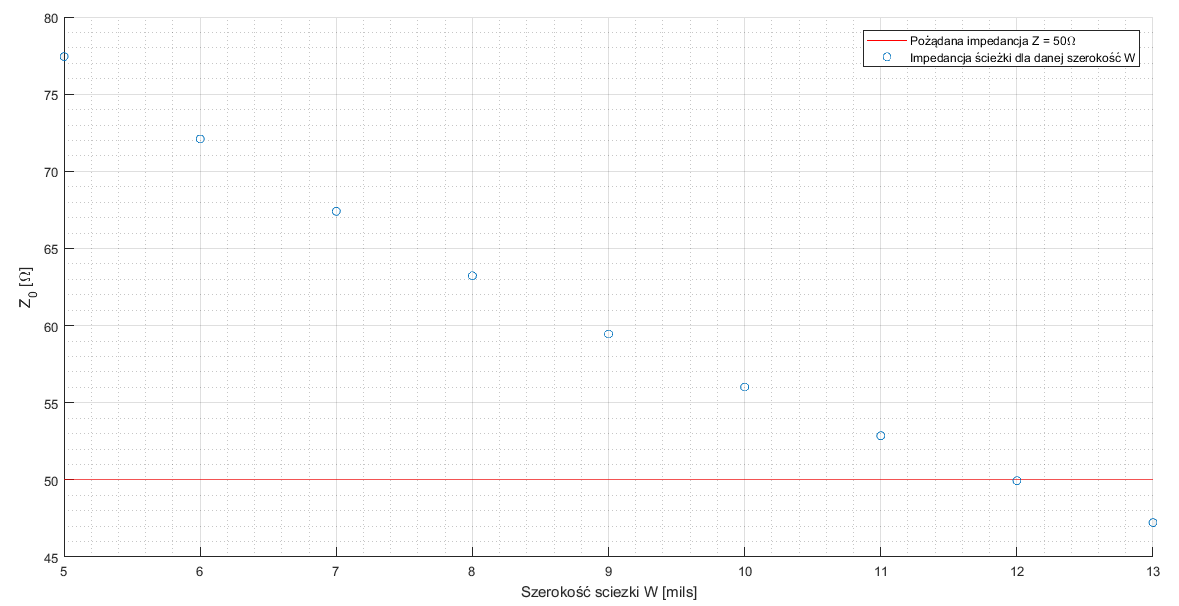
\includegraphics[width=\textwidth]{plots/gpsZ0.png}
    \caption{\textit{\scriptsize Impedancja ścieżki w zależności od szerokości ścieżki}}
\end{figure}

Powyższy wykres przedstawia impedancję ścieżki w zależności od szerokości dla anteny modułu GPS obliczoną ze wzoru ~\ref{eq:gps_z0} z parametrami $T = 1,4 mils$ i $H = 6,7 mils$ wziętymi z tabeli ~\ref{tab:pcbStack}. Czerwoną linią zaznaczono pożądane dopasowanie $Z_0 = 50 \Omega$. Założono że W zostanie obliczone z dokładnością do 1 mils. Obliczenia wykonano zaczynając od najmniejszej szerokości gwarantowanej przez producenta $W = 5 mils$, aż do punktu pod prostą z optymalnym dopasowaniem. Najlepsze dopasanie otrzymano dla $W = 12 mils$, gdzie $Z_0 \approx 49.95$
Dla takiego $Z_0$ obliczono współczynnik odbicia, który reprezentuje jaka część sygnału została stracona w wyniku niedopasowania impedancji przy przejściu pomiędzy liniami transmisyjnymi.

\begin{equation}
\Gamma= \frac{Z_l - Z_s}{Z_l + Z_s} \label{eq:gammaGPS}
\end{equation}
gdzie
\begin{itemize}
  \item $Z_l$ - impedancja obciążenia, w tym przypadku impedancja lini transmisyjnej $Z_0 = 49,95 \Omega$
  \item $Z_s$ - impedancja źródła, czyli wejścia antenowego modułu GPS, zgodnie z notą katalogową $Z_s = 50 \Omega$
\end{itemize}

Korzystając ze wzoru ~\ref{eq:gammaGPS} obliczono:
\begin{equation}
\Gamma= \frac{Z_0 - Z_s}{Z_0 + Z_s} = \frac{49,59\Omega -50\Omega}{49,59\Omega  + 50\Omega } \approx 0.0005
\end{equation}

W przeliczeniu na procenty daje to $\Gamma \cdot 100\% = 0.0005 \cdot 100\% = 0.05\%$ sygnału odbitego przez linie transmisyjną. Jest to wartość akceptowalna zatem pozostano prze szerokości $W = 12 mils$.\\

Zgodnie z zaleceniami noty katalogowej wykonano serię przelotek pod i do okola układu GPS (U2). Ten sam zabieg zastosowano również dla ścieżki antenowej (pomiędzy J1 i U2). Zapewniło to lepsze odprowadzanie ciepła przez moduł, a zatem niższą temperaturę pracy i mniejsza emisję EMC. Poniżej zaprezentowano zdjęcie z projektem.
\begin{figure}[!h]
    \centering
    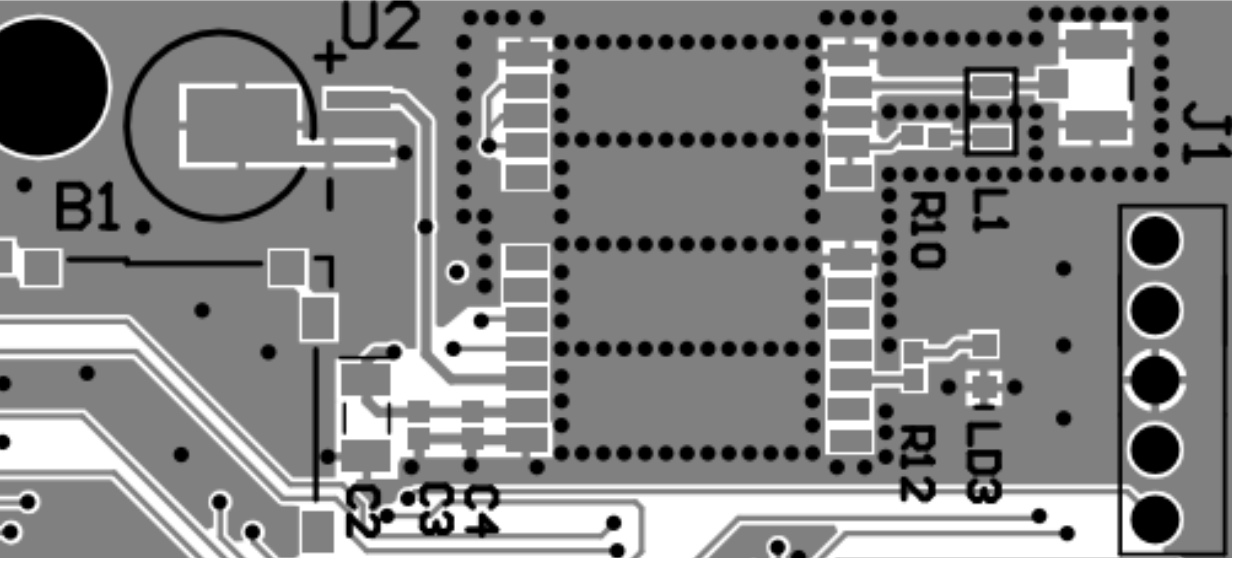
\includegraphics[width=15cm]{pcb/gps.png}
    \caption{\textit{\scriptsize Projekt PCB dla GPS}}
\end{figure}

\subsection{USB}
W projekcie wykorzystano wbudowany w mikrokontroler kontroler interfejsu USB2.0 High-Speed o maksymalnej przepustowości 12Mb/s. Zgodnie ze standardem, należy dopasować impedancję różnicową pomiędzy liniami transmisyjnymi sygnału nieodwróconego i odwróconego do 90 \textbf{$\Omega$}. Poniżej przedstawiono zastosowany wzór oraz obliczenia.
\begin{equation}
Z_0= \frac{174}{\sqrt{\varepsilon_r + 1.41}}\ln{\left(\frac{5.98H}{0.8W + T}\right)} \left(1-0.48e^{(-0.96\frac{D}{H})}\right) \label{eq:usb_zd}
\end{equation}
dla 
$$
0,1 < W/H < 2,0
$$
$$
1 < \varepsilon_r < 15
$$
gdzie
\begin{itemize}
  \item \textbf{$\varepsilon_r$} - stała dielektryczna
  \item H - grubość dielektryka
  \item W - szerokość ścieżki
  \item T - grubość ścieżki
  \item D - odległość pomiędzy ścieżkami
\end{itemize}

\begin{figure}[!h]
    \centering
    \includegraphics[width=\textwidth]{plots/usbzD.png}
    \caption{\textit{\scriptsize Impedancja różnicowa w zależności od szerokości ścieżki}}
\end{figure}

Poniższy wykres przedstawia impedancję różnicową lini transmisyjnych interfejsu USB w zależności od szerokości obliczoną ze wzoru ~\ref{eq:usb_zd} z parametrami $T = 1,4 mils$ i $H = 6,7 mils$ wziętymi z tabeli ~\ref{tab:pcbStack}. Założono odległość pomiędzy ścieżkami $ D = 8mils$ równą rozstawowi padów w mikrokontrolerze. Czerwoną linią zaznaczono pożądane dopasowanie $Z_d = 90 \Omega$. Założono że W zostanie obliczone z dokładnością do 1 mils. Obliczenia wykonano zaczynając od najmniejszej szerokości gwarantowanej przez producenta $W = 5 mils$, aż do punktu pod prostą z optymalnym dopasowaniem. Najlepsze dopasanie otrzymano dla $W = 11 mils$, gdzie $Z_d \approx 89.56$. Zgodnie ze specyfikacją interfejsu USB2.0 Full-speed (12 Mb/s) impedancja różnicowa musi wynosić $Z_d = 90 \pm 15\%$. Zatem $ 76,5\Omega <= Z_d <= 103,5\Omega$. $Z_d$ obliczone dla $W = 11mils$ spełnia to wymaganie.

Wszystkie elementy zostały umieszczone na górnej warstwie sygnałowej, aby nie stosować przelotek które wprowadzając niepożądane pojemności i indukcyjności linii transmisyjnym. Ścieżki są zaginane po kątem nie większym niż 45$^\circ$.Warstwą referencyjną dla sygnałów jest warstwa masy co zapewnia lepsze ekranowanie dla sygnałów szybkich. Linie różnicowe są oddzielone polem masy od innych sygnałów o co najmniej 50mils (1.27mm). Zastosowanie powyższych reguł pozwoliło ograniczyć zjawiska utrudniające dopasowania impedancji. Wspominanie w rozdziale schematu rezystory R5 i R4 służą jako szeregowa terminacja sygnału. Dzięki temu zabiegowi czasy narastania zboczy się większe co zmniejsza generowanie zakłócenia EMC. Układ U6 działa jako zabezpieczenie przeciwko wyładowaniom elektrostatycznym mogącym uszkodzić urządzenie oraz jako dodatkowy filtr EMC.Zgodnie z notą katalogową katalogową układu STM32F767xx ich rezystancja wynosi 22 \textbf{$\Omega$}. Poniżej przedstawiono część projektu PCB z interfejsem USB.

\begin{figure}[!h]
    \centering
    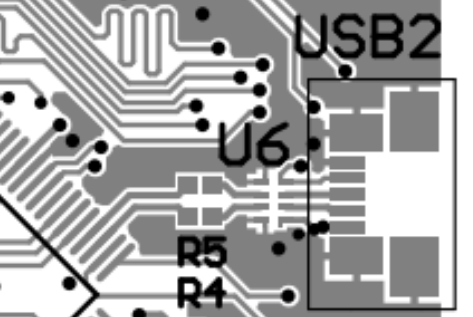
\includegraphics[width=9cm]{pcb/usb.png}
    \caption{\textit{\scriptsize Projekt PCB dla interfejsu USB}}
\end{figure}

\subsection{Interfejsy szybkie}
Częstotliwość sygnału zegarowego FMC wynosi $108Mhz$. W przypadku komunikacji z wyświetlaczem szybkość interfejsu zależy od oczekiwanej liczby klatek na sekundę. Częstotliwość sygnału zegarowego dla interfejsu MIPI-DPI wyraża się wzorem:
\begin{equation}
CLK = W \cdot H \cdot fps \label{eq:fps}
\end{equation}
gdzie:
\begin{itemize}
  \item W - szerokość matrycy w pikselach
  \item H - wysokość matrycy w pikselach
  \item fps - częstotliwość odświeżania ekranu
\end{itemize}
Dla użytego w projekcie wyświetlacza przy założeniu odświeżania matrycy 60Hz korzystając z równania ~\ref{eq:fps} otrzymujemy:
$$
CLK = 1024 \cdot 600 \cdot 60Hz = 614400 \cdot 60Hz = 36864000 Hz \approx 37MHz
$$
Interfejsy o takich częstotliwościach zostały uznane za szybkie, co za tym idzie podjęto dodatkowe działania podczas projektowania ich linii transmisyjnych. Zadbano by warstwy referencyjne pod ścieżkami sygnałowymi były ciągłe, aby zapewnić ekranowanie i ograniczyć przesłuchy od linii po przeciwnej stronie płytki. Ponadto dopasowano długości wszystkich ścieżek w interfejsie, by sygnały przychodziły w tym możliwie podobnym czasie. Wzorując się na projekcie referencyjnym płytki ewaluacyjnej STM32F746G-DISCO zadbano, by różnica długości pomiędzy ścieżkami dla obu interfejsów nie była większa niż $100 mils$.Opóźnienie linii transmisyjnej, czyli czas jaki sygnał potrzebuje na pokonanie określonej drogi wyraża się wzorem:
\begin{equation}
t = \frac{l \sqrt{\varepsilon_r}}{c} \label{eq:td}
\end{equation}
gdzie
\begin{itemize}
  \item l - długość linii transmisyjnej
  \item \textbf{$\varepsilon_r$} - stała dielektryczna 
  \item c - szybkość rozchodzenia się fali w próżni
\end{itemize}
Korzystając ze wzoru ~\ref{eq:td} dla parametrów $l = 0.00254m$ $(100 mils)$ i $c = $ $299$ $792$ $458\frac{m}{s}$ oraz $\varepsilon_r =3,66$ obliczono opóźnienie sygnału czyli maksymalny odstęp czasu w jakim dzieli sygnały w liniach o długości różniącej się o $100mils$.
$$
t = \frac{0.00254m \sqrt{3,66}}{299 792 458\frac{m}{s}} = \frac{0.00485931m}{299 792 458\frac{m}{s}} = 1.621\cdot10^-11 = 16,21 ps
$$

Wyświetlacz jest sterowny bezpośrednio poprzez interfejs LVDS (ang. Low Voltage Differential Signaling), jednak  posiada również wbudowany konwerter THC63LVDM83D pozwalający na komunikację ze pomocą MIPI-DPI. Oznacza to, że wszelkie ograniczenia czasowe powinny być rozpatrywane względem wspomnianego wcześniej układu. Wyjścia
mikrokontrolera zmieniają się przy zboczu opadającym sygnału zegarowego, natomiast są zatrzaskiwane przez konwerter przy zboczu narastającym. Wszystkie sygnały powinny dojść do wyświetlacza od momentu wystąpieniem zbocza opadającego do narastającego z uwzględnieniem czasu ustalenia się sygnału (ang. Setup Time). Jest to najpóźniejszy moment w którym muszą ustalić się stany na wszystkich liniach przed przyjściem sygnału taktującego. Poniżej przedstawiono diagram ilustrujący opisane ograniczenia czasowe.

\begin{figure}[!h]
    \centering
    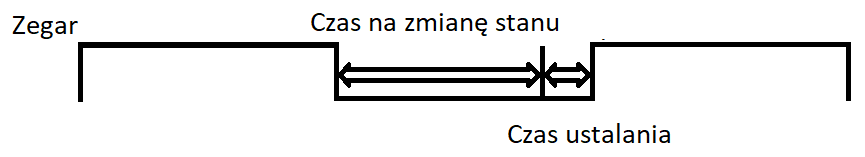
\includegraphics[width=10cm]{plots/timing.png}
    \caption{\textit{\scriptsize Diagram ograniczeń czasowych}}
\end{figure}

Zatem maksymalna rozbieżność czasowa pomiędzy sygnałami wyraża się wzorem.
\begin{equation}
t_{max} = t_{low}- t_{setup} \label{eq:timing}
\end{equation}
gdzie
\begin{itemize}
  \item \textbf{$t_{low}$} - czas trwania stanu niskiego dla sygnału zegarowego
  \item \textbf{$t_{setup}$} - czas ustalania dla sygnału
\end{itemize}

Z noty katalogowej mikrokontrolera odczytano że stan niski dla sygnał zegarowego LTDC wynosi minimalnie $45\%$
okresu sygnału zegarowego obliczonego z równania ~\ref{eq:fps}zatem:
$$
t_{low} = \frac{1}{36864000Mhz} \cdot 45\% = 27127ps\cdot45\% = 12207ps
$$
W nocie THC63LVDM83D znaleziono $t_{setup} = 2000ps$. Korzystając z ~\ref{eq:timing} obliczono
$$
t_{max} = 4167ps - 2000ps = 2167ps
$$
Ograniczenia czasowe nie zostały przekroczone, ponieważ $t_{max}= 12207ps >= t=16,21$.\\

W przypadku FMC wykorzystywanego do obsługi SDRAM, komunikacja odbywa się w obie strony. Ponownie czas trwania stanu niskiego sygnału zegarowego wynosi $45\%$ okresu. Zatem:
$$
t_{low} = \frac{1}{108Mhz} \cdot 45\% = 9259ps\cdot45\% = 4167ps
$$
 Poniżej przedstawiono tabelę z czasami ustalania dla wszystkich sygnałów interfejsu odczytanych z noty ukłądu IS42S16400J-7TLI.

\begin{table}[htb]

\caption{\textit{ Czasy ustalania dla wszystkich sygnałów układu SDRAM}}
\label{tab:sdramTiming}
\begin{center}
\begin{tabular}{ |c|c| }
\hline
Parametr  & czas [ps] \\ 
\hline
Input Data Setup Time & 1500 \\ 
\hline
Address Setup Time & 1500\\ 
\hline
CKE Setup Time	 & 1500\\ 
\hline
Command Setup Time	 & 1500\\ 
\hline
\end{tabular}
\end{center}
\end{table}

Oznacza to, że można przyjąć $t_{setup}=1500ps$. Korzystając z równania ~\ref{eq:timing} obliczono:
$$
t_{max} = 4167ps - 1500ps = 2667ps
$$
Ponownie $t_{max}= 2667ps >= t=16,21$, zatem ograniczenia czasowe nie zostały przekroczone.


Poniżej przedstawiono zbliżenie na projekt PCB, gdzie można zauważyć meandry na ścieżkach,których celem jest wyrównanie różnicy długości pomiędzy ścieżkami sygnałowymi.

\begin{figure}[!h]
    \centering
    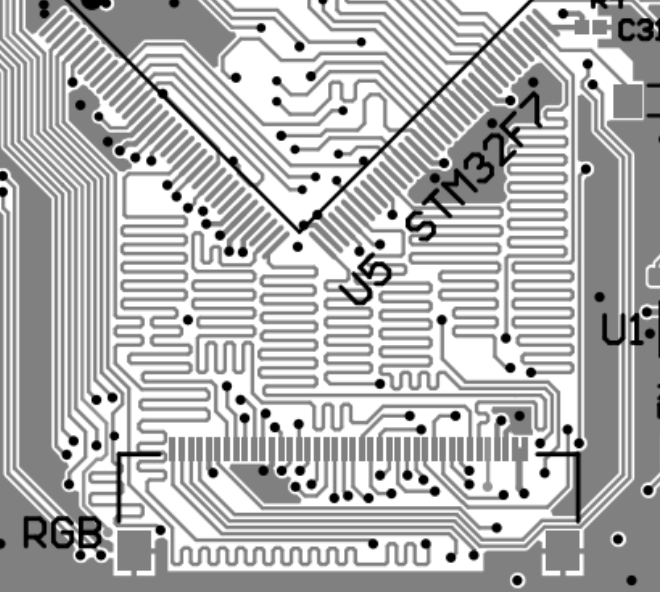
\includegraphics[width=\textwidth]{pcb/ltdc.png}
    \caption{\textit{\scriptsize Przykład dopasowania długości ścieżek na PCB}}
\end{figure}

\subsection{Warstwa zasilania}
Większość układów na PCB jest zasilana napięciem 3,3V. Jednak interfejs USB i podświetlenie wyświetlacza wymaga napięciem 5V. Wymagało to odpowiedniego podzielania warstwy trzeciej. Zadbano o to żeby żadne ścieżki sygnałów wrażliwych na zakłócenia nie przechodziły nad przerwą pomiędzy polem zasilanie 3,3V i 5V. Nieciągłość warstwy referencyjne powoduje powstawanie pętli prądowych, ponieważ prąd powrotny szuka innej dostępnej ścieżki powrotu. Zjawisko to może powodować wzrost zakłóceń elektromagnetycznych emitowanych przez urządzenie. Warstwę przedstawia obraz ~\ref{fig:power} w podrozdziale \ref{pcbOverview}.
\subsection{Prezentacja PCB} \label{pcbOverview}
Poniżej przedstawiano obrazy wszystkich warstw z programu wykorzystanego do projektu oraz zdjęcie gotowego PCB.
\begin{center}\centering
\vspace*{\fill}
\begin{figure}[!h]
    \centering
    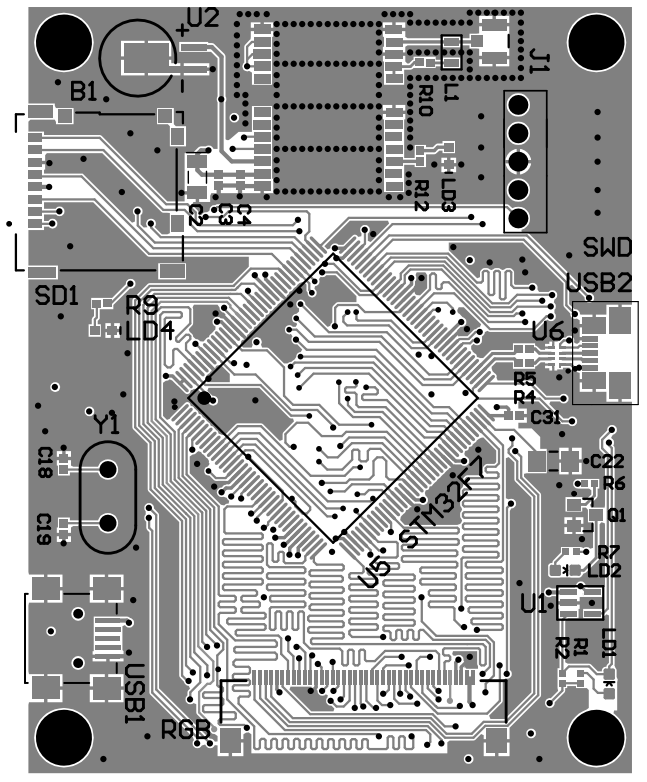
\includegraphics[width=\textwidth]{pcb/top.png}
    \caption{\textit{\scriptsize Układ warstwy 1.}}
\end{figure}
\vfill
\end{center}
\newpage

\begin{center}\centering
\vspace*{\fill}
\begin{figure}[!h]
    \centering
   	
    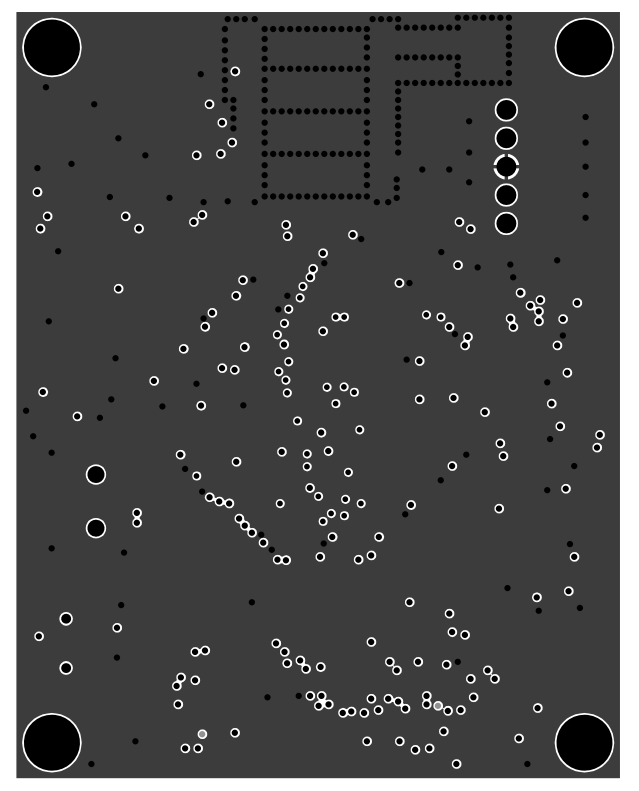
\includegraphics[width=\textwidth]{pcb/gnd.png}
    \caption{\textit{\scriptsize Układ warstwy 2.}}
\end{figure}
\vfill
\end{center}
\newpage

\begin{center}\centering
\vspace*{\fill}
\begin{figure}[!h]
    \centering
    \label{fig:power}
    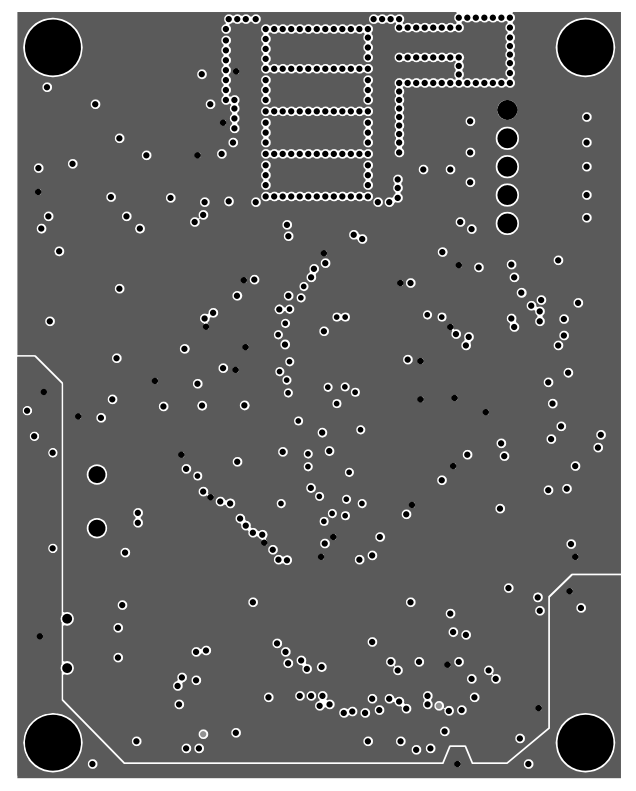
\includegraphics[width=\textwidth]{pcb/power.png}
    \caption{\textit{\scriptsize Układ warstwy 3.}}
\end{figure}
\vfill
\end{center}
\newpage

\begin{center}\centering
\vspace*{\fill}
\begin{figure}[!h]
    \centering
    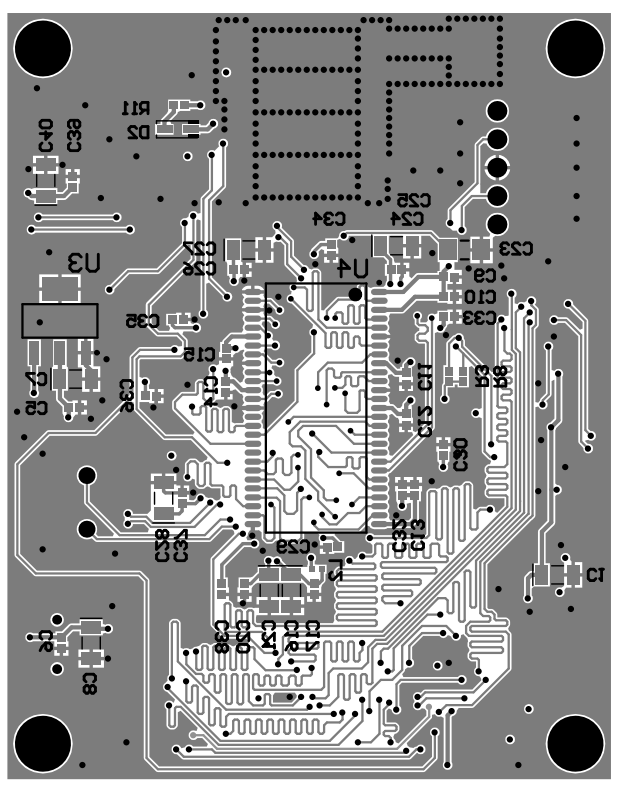
\includegraphics[width=\textwidth]{pcb/bottom.png}
    \caption{\textit{\scriptsize Układ warstwy 4.}}
\end{figure}
\vfill
\end{center}
\newpage

\section{Architektura systemowa}
\chapter{ Podsumowanie }


\addcontentsline{toc}{chapter}{Bibliografia} %utworzenie w spisie treści pozycji Bibliografia
\bibliography{bibliografia} % wstawia bibliografię korzystając z pliku bibliografia.bib - dotyczy BibTeXa, jeżeli nie korzystamy z BibTeXa należy użyć otoczenia thebibliography

%opcjonalnie może się tu pojawić spis rysunków i tabel
% \listoffigures
% \listoftables
\end{document}
